\chapter{Wdrożenie i testy}
\label{cha:rozdzial6}

\begin{itemize}
\item Opis instalacji i uruchamiania programu klienta
\item Opis przeprowadzonych testów działania/testów porównawczych
\item Pokazanie w jaki sposób skonfigurować sieć lokalną (multicasty) w celu zmniejszenia jej obciążenia przy transmisjach jeden-do-wielu. Tylko klient DASH łączy się do serwera. Pozostałe komputery w sieci kampusowej odbierają transmisję od klienta DASH.
\begin{center}
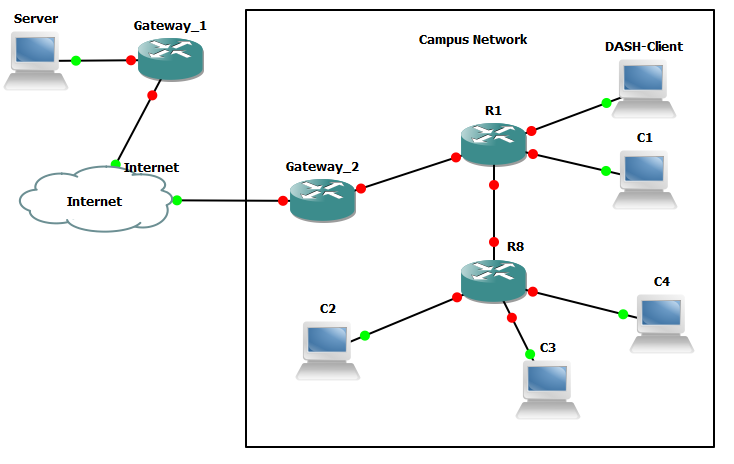
\includegraphics[scale=0.7]{lan}
\end{center}
\end{itemize}